\chapter{Anatomical correlations in the femur}
\label{ch:version}

\section{Abstract}
\label{sec:version_abstract}
Femoral version, or twist angle, is an important gross anatomical feature of the femur.
It has relevance to mechanical testing, falls analysis and surgery of the proximal femur.
In order to determine version using traditional methods, access to the entire bone, either by direct inspection or through imaging, is require.
In some cases this is not possible.
An investigation of the relationship between femoral version and the linea aspera angle at the shaft 50\% length was conducted, searching for a correlation that would allow version determination from the inspection of only the proximal half of the femur.
\acs{3d} surface scans of 14 femurs were obtained and the version, posterior neck, and linea aspera angles were measured using the digital models.
The version and posterior neck angles were found to be moderately correlated ($R^2 = 0.52$), with a regression coefficient near unity.
The version and linea aspera angles were found to be moderately correlated ($R^2 = 0.48$), with a regression coefficient of near negative one.
These results indicate that an approximation of a femur's version angle can be found by evaluating the angle that separates linea aspera at the 50\% length position and the femoral neck.
This result has implications in mechanical testing of proximal femora and orthopaedic surgery when the angle of the femoral neck must be determined without access to either the proximal or distal end of the bone.

\section{Introduction}
\label{sec:version_intro}
Fractures of the proximal femur are common and debilitating injuries.
They are associated with a high level of morbidity and mortality and are estimated to cost the US health care system nearly \$2 billion each year~\citep{abrahamsen_excess_2009, song_cost_2011}.
Critical to preventative screening for such injuries is an understanding of the fracture mechanics, which are ideally observed under conditions mimicking those experienced during a real fall to the side.

Previous femoral fracture researchers recognized that one of the most critical aspects the testing was orientation of the femur to the loading vector~\citep{pinilla_impact_1996, backman_proximal_1957, ford_effect_1996}.
It was observed that changing the orientation could lead to changes in fracture load equivalent to multiple decades of bone mineral loss~\citep{pinilla_impact_1996, ford_effect_1996}.
To control for this, injury biomechanists developed a standard loading orientation which was defined as 10$^\circ$ of adduction of the shaft and 15$^\circ$ of internal rotation of the neck (Fig.~\ref{fig:version_Constraints})~\citep{courtney_age-related_1995, de_bakker_during_2009, courtney_effects_1994, manske_femoral_2006, lochmuller_mechanical_2002, backman_proximal_1957}.

\begin{figure}
\centering
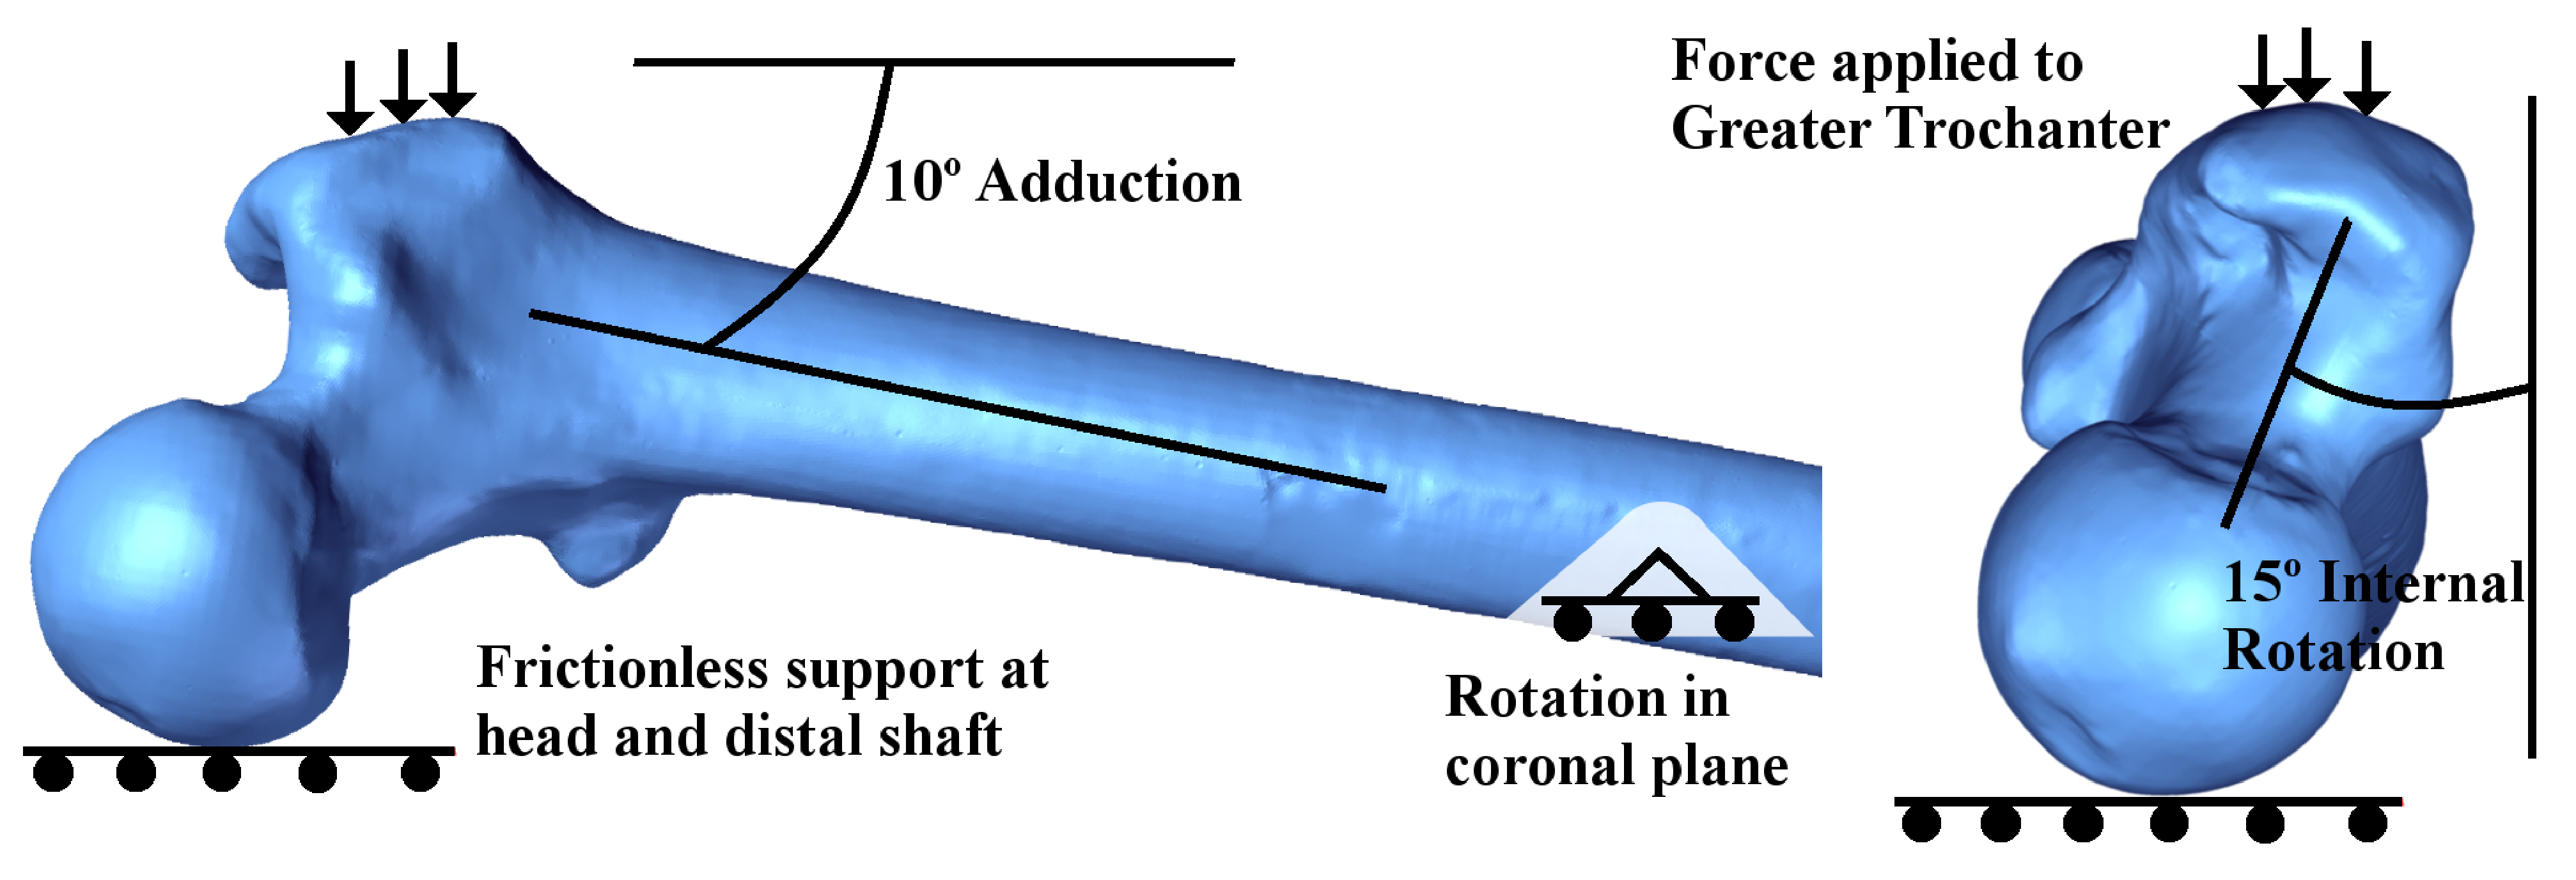
\includegraphics[width=\linewidth]{./appendixVersion/figures/FEM_Constraints}
\caption[Constraints and orientation]{\textbf{Constraint and orientation of the proximal femur during mechanical testing. Anterior on the left and superior on the right.} Graphic \copyright Seth Gilchrist, 2013.}
\label{fig:version_Constraints}
\end{figure}


Standardization of the proximal femur orientation can be thought of as standardizing the fall being modelled.
Fall researchers have shown that, in falls to the side, the impact happens at a location that can be characterized with reference to the mid-coronal plane~\citep{feldman_reducing_2007}.
If the orientation of the leg during a fall is determined by lower limb position, then using the femoral neck to orient the proximal femur during fall simulation would effectively of model a different leg position for each specimen as the angle of the femoral neck varies widely in the general population~\citep{toogood_proximal_2009}.
This fact presents a potential limitation in study of femoral fractures through laboratory fall simulation.
Some specimens may display significantly different fracture characteristics, and researchers currently cannot determine if this was due to the fall being modelled.
If the orientation of the femoral neck relative to the coronal plane in life could be ascertained on a specimen-by-specimen basis, a more generalized method for orienting the proximal femur during testing, or identifying bones with extreme anatomical characteristics, might be feasible.

Femoral version is the acute angle made by the axis of the femoral neck with the femoral plane (Figs.~\ref{fig:Planes} and~\ref{fig:Version}).
Since the femoral plane and coronal plane are approximately coincident~\citep{matsuda_femoral_1998, matsuda_anatomical_2004}, knowledge of the femoral version could allow researchers greater ability to determine the fall being modelled in each test.
Researchers who study proximal femur fracture often work with only the proximal femur and do not have access to the distal end, which is required for determination of femoral version.
In these cases, knowledge of the femoral version would need to be determined based solely on proximal femur landmarks.
The linea aspera angle was selected as a potential proximal landmark as it is the insertion of both proximal and distal muscles and its location may be dictated by femoral version.

The goal of the current study was to determine if the angle of the femoral neck and the angle of the linea aspera at 50\% shaft length could be used to determine femoral version.
If the angle of the linea aspera at 50\% shaft length is influenced by the femoral version, then knowledge of the angle between the femoral neck and the linea aspera may be able to inform specimen version without access to the femoral condyles.
Thus, we hypothesised that the angle between the femoral neck and the linea apsera at 50\% shaft length would be correlated with femoral version.

\section{Materials and methods}
\label{sec:version_methods}
15 femurs were obtained from the historical bone collection at \acs{ubc}, Department of Anatomy.
The bones surfaces were scanned using a \ac{3d} laser scanner (Vivid i9, Konica-Minolta, Ramsey, NJ).
Because the bones were too long to fit into the field of view of the scanner, they were scanned in two parts, proximal and distal.
Fiducial markers made of modelling clay were fixed to the bone surface to aid in registering of the two halves during \ac{3d} modelling (Fig.~\ref{fig:version_setup}).
The bones were mounted on a rotary table and 9 scans in 40$^\circ$ increments were made of each end.

\begin{figure}
\centering
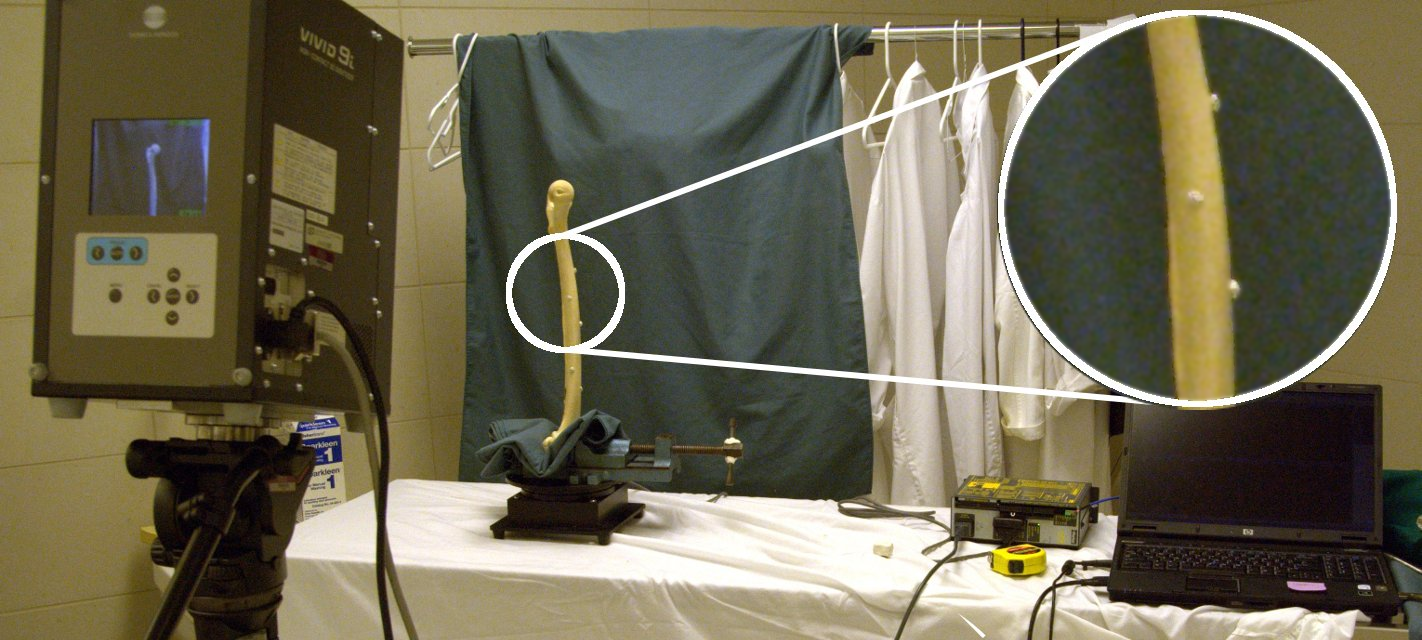
\includegraphics[width=0.7\linewidth]{./appendixVersion/figures/setup}
\caption[Femur scanning set up]{\textbf{An image of the scanning set up. The femur is mounted on a software controlled rotary table. Each end of the femur was scanned independently and the scans were aligned with the aid of fiducial markers on the shaft, visible in the insert.} Image \copyright Seth Gilchrist, 2013.}
\label{fig:version_setup}
\end{figure}

The scans were imported into \ac{3d} modelling software (RapidForm XOR3, INUS Technology, Seoul, South Korea) where they were aligned, merged and cleaned.
The femoral plane was defined by creating a surface that contacted the posterior femoral condyles distally and the trochanter proximally.
The condyler plane as defined as perpendicular to the femoral plane, contacting both inferior condyles, and the third plane was defined as perpendicular to the other two, passing through the femoral head (Fig.~\ref{fig:Planes}).
Measurements of the \ac{av} and \ac{apn}were made using the femoral plane for reference, while the \ac{ala} measurements used the third plane for reference.

Version measurement was performed using a technique based on the method developed by \citet{kingsley_study_1948}, adapted for the virtual environment (Fig.~\ref{fig:version_version}).
To our knowledge, no standard protocols exist for measurement of the posterior neck (Fig.~\ref{fig:version_pn}) or linea aspera (Fig.~\ref{fig:version_la}) angles, and as such a new methods were required.

\begin{figure}
\centering
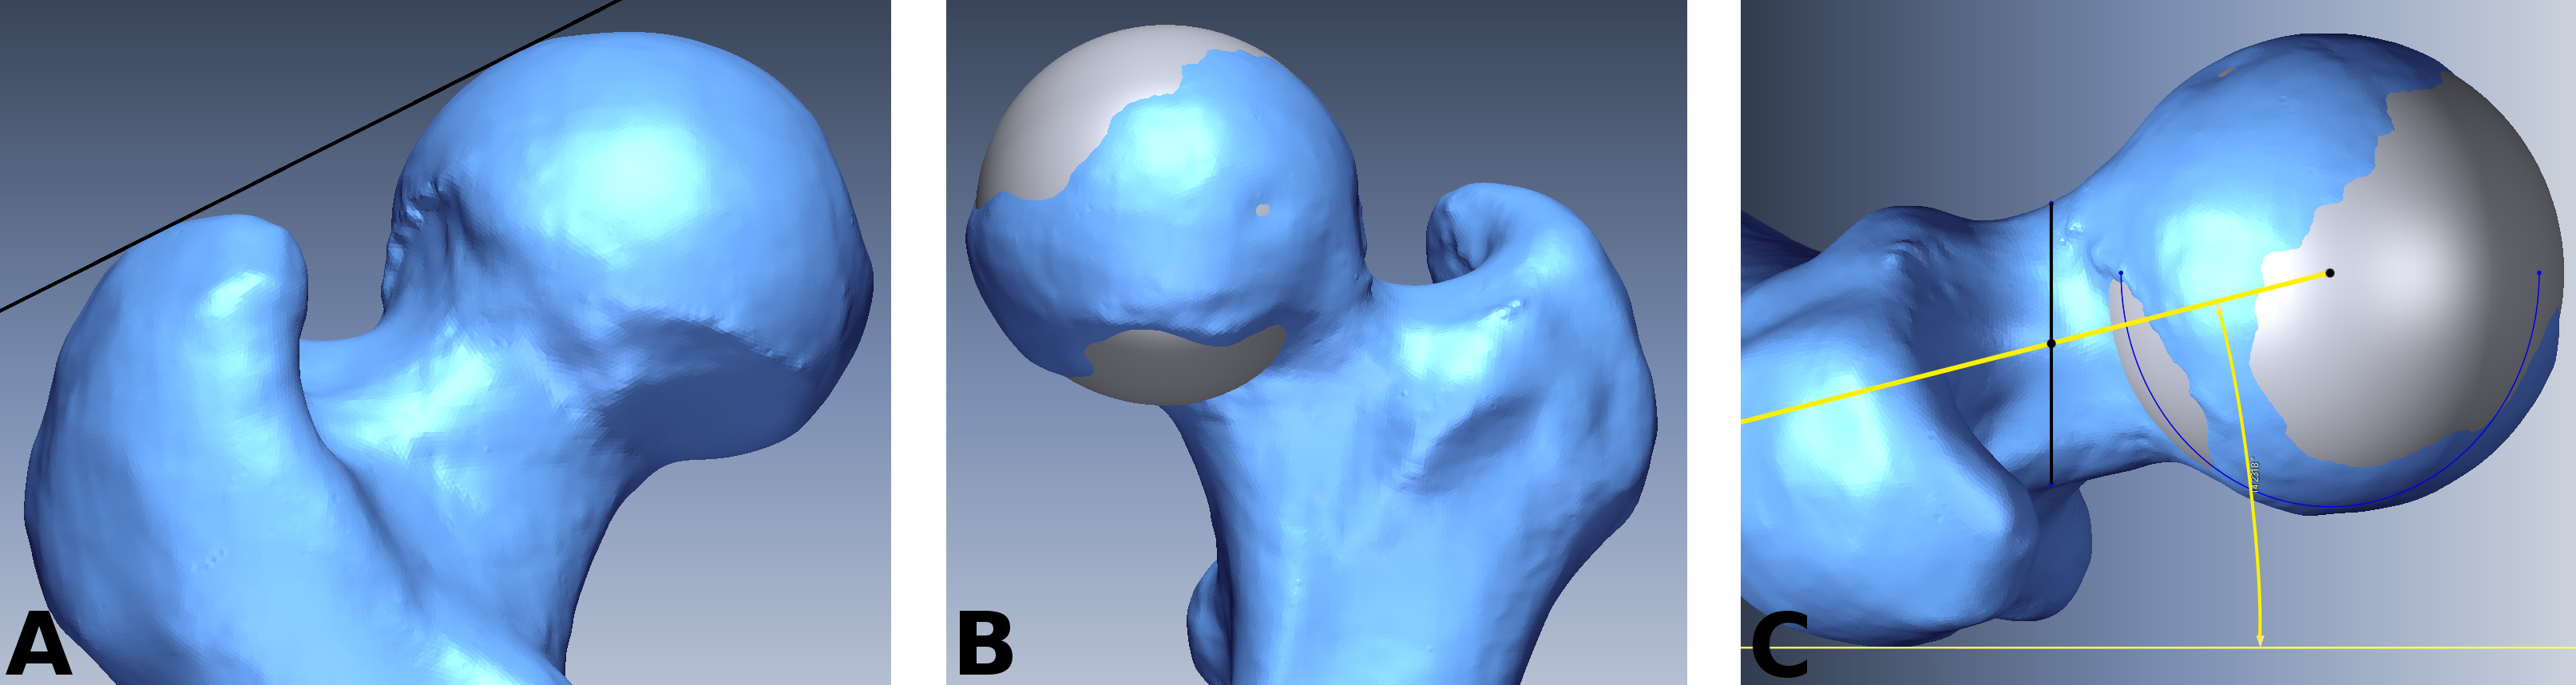
\includegraphics[width=\linewidth]{./appendixVersion/figures/version}
\caption[Digital version measurement]{
\textbf{Version was measured in four steps. A plane perpendicular to the femoral plane, contacting the head and greater trochanter was defined (A). A sphere was fit to the femoral head to locate its centre (B). The view was aligned perpendicular to the plane defined in (A) and two lines were drawn. One was perpendicular to the femoral plane and across the femoral neck. The second was from the centre of the femoral head to the midpoint of the previously drawn line (C). The acute angle from the femoral plane to the second line defined the version of the specimen. Anterior version was taken as positive.} Graphic \copyright Seth Gilchrist, 2013.}
\label{fig:version_version}
\end{figure}

\begin{figure}
\centering
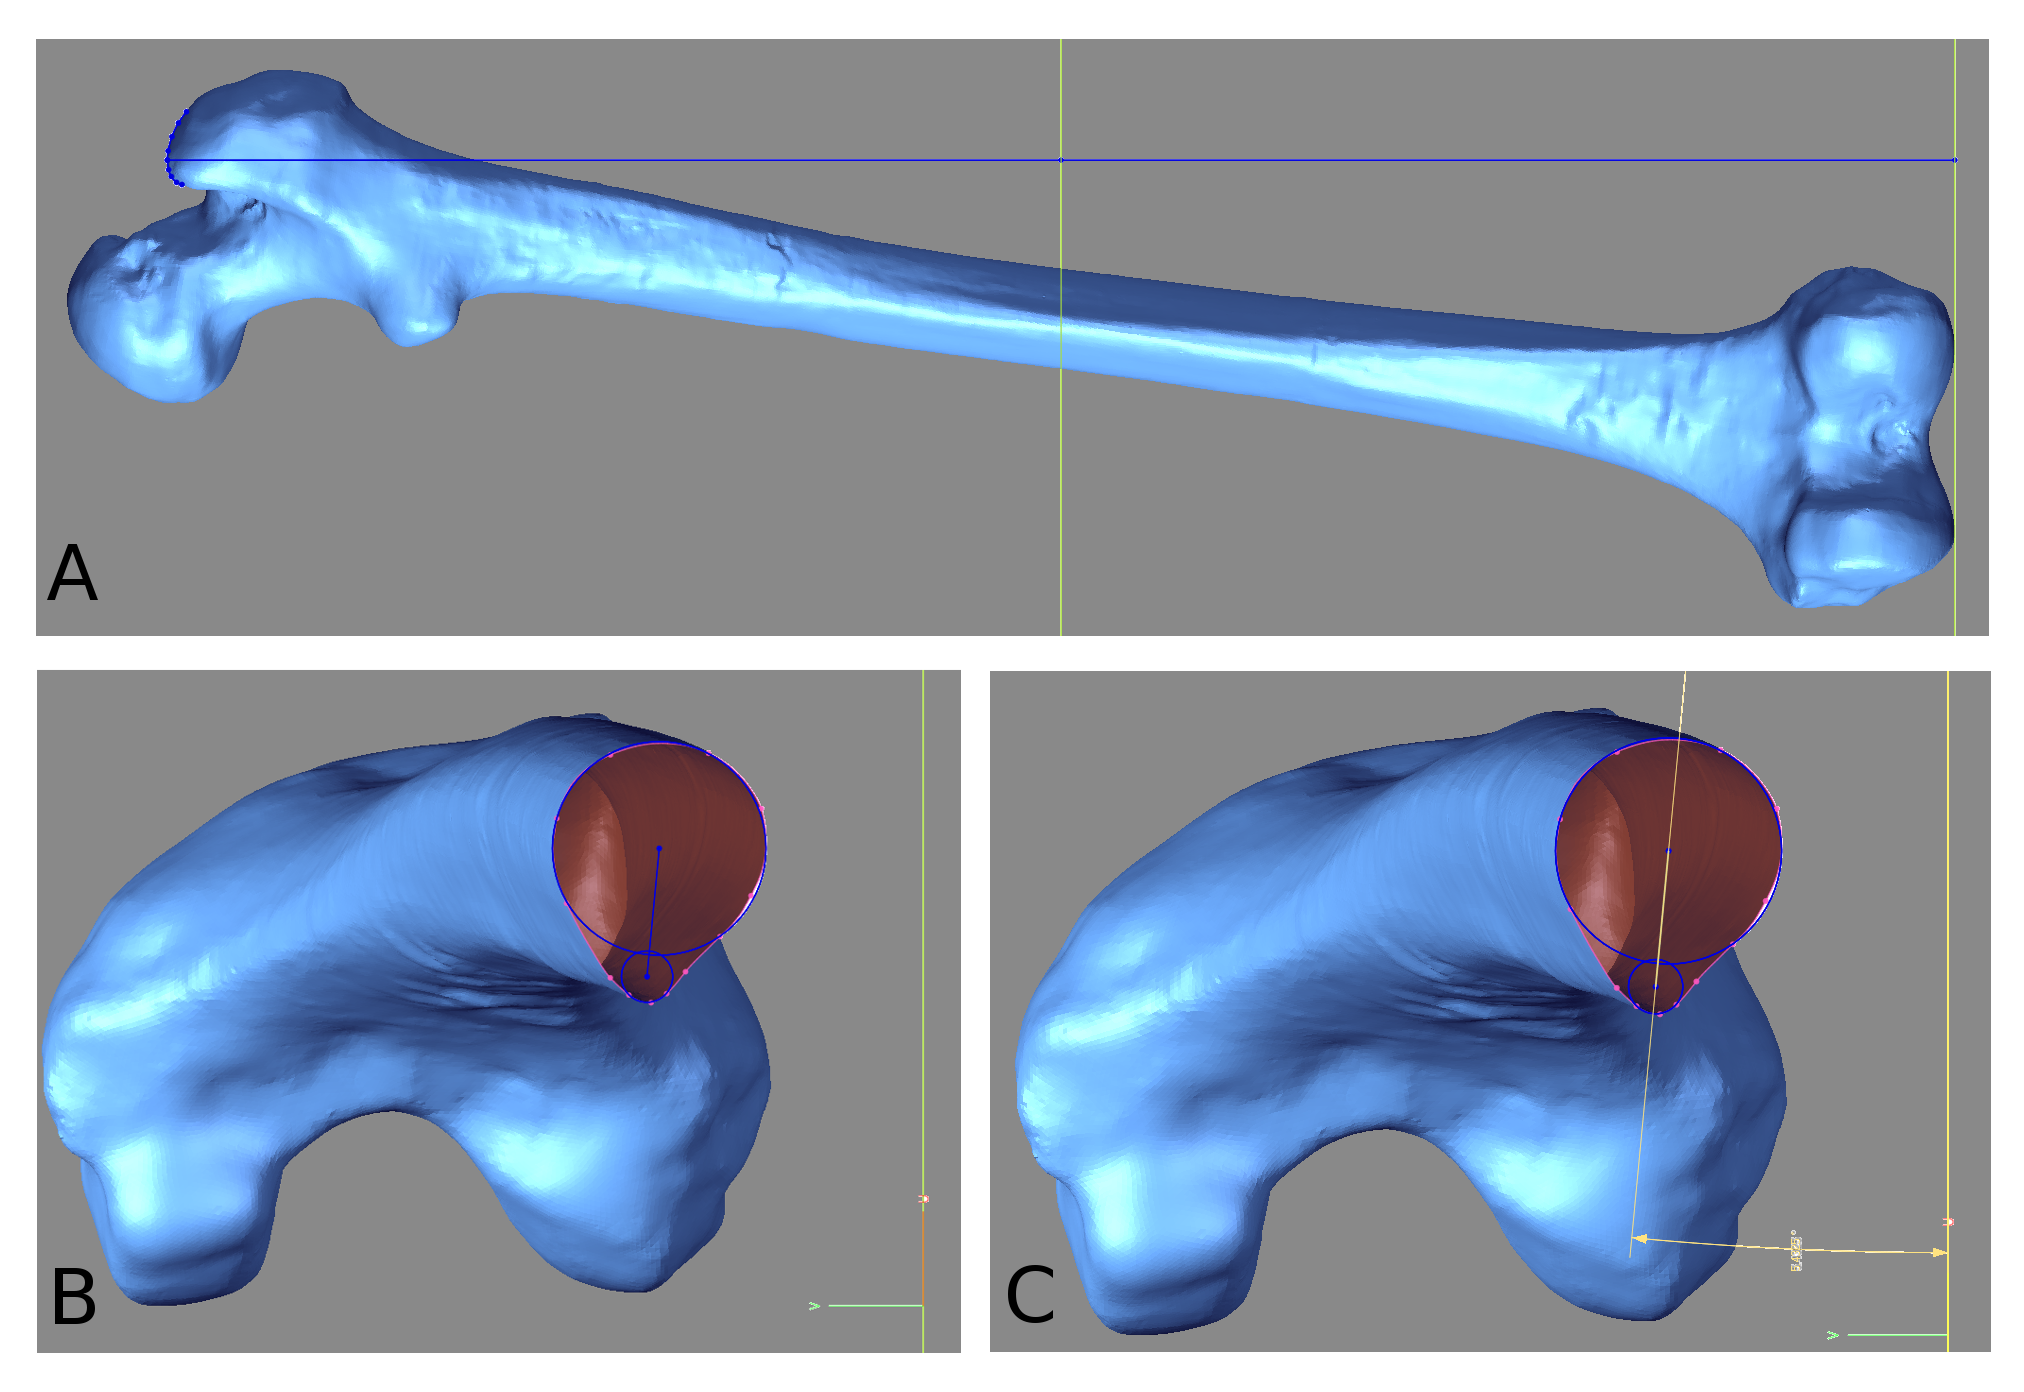
\includegraphics[width=0.7\linewidth]{./appendixVersion/figures/la}
\caption[Digital linae aspera measurement]{
\textbf{Linea aspera measurements were conducted in three steps. The proximal end of the femur was masked out at the 50\% shaft location (A). Two circles were defined, one was fit to the entire shaft cross section, and the other defined using the posterior prominence of the linea aspera (B). A line was drawn through the centres of both circles, and the acute angle of this line with the third plane was the linea aspera angle (C). Medial rotation was taken as positive.} Graphic \copyright Seth Gilchrist, 2013.}
\label{fig:version_la}
\end{figure}

\begin{figure}
\centering
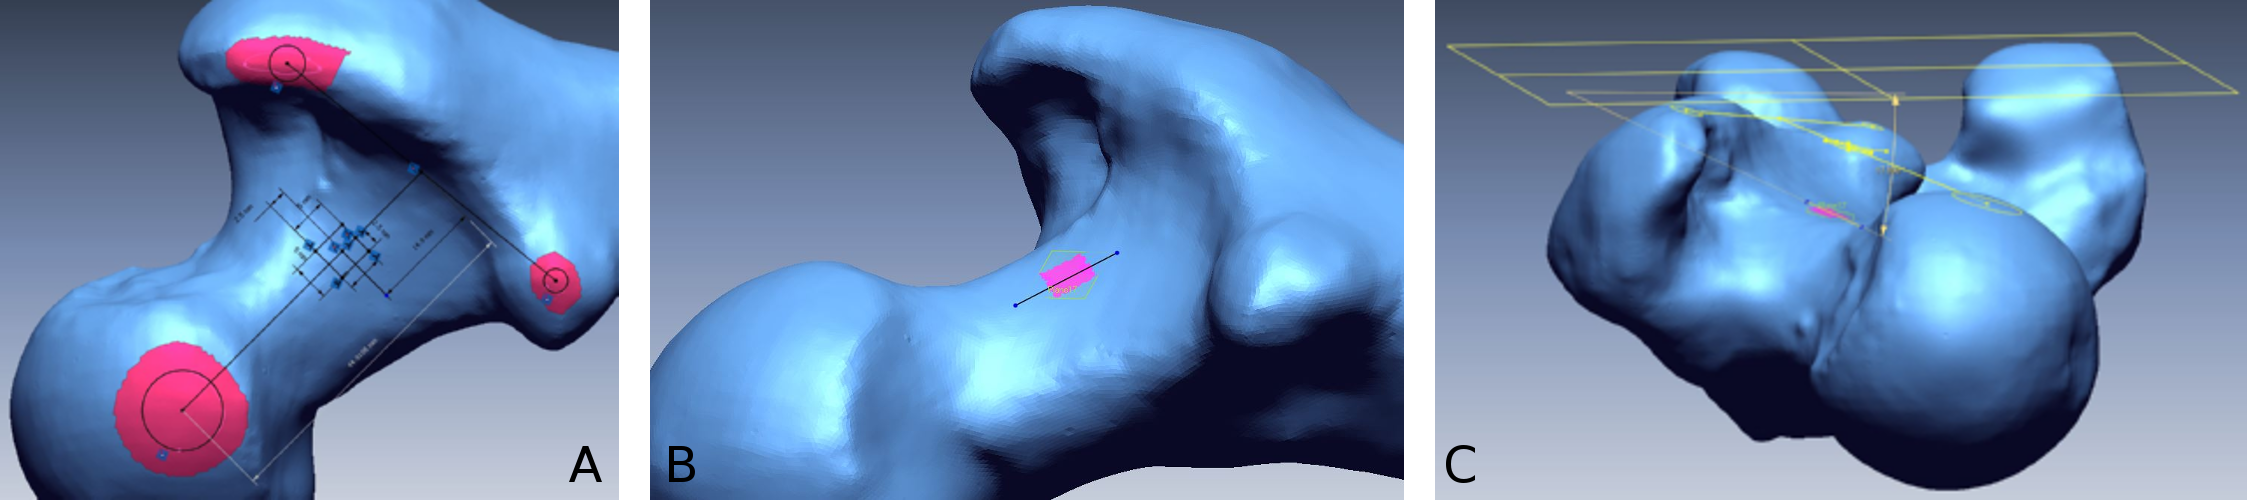
\includegraphics[width=\linewidth]{./appendixVersion/figures/pn}
\caption[Digital posterior neck measurement]{
\textbf{The posterior neck angle measurement was done in four steps. A plane was defined that touched the posterior head and trochanters. Drawn on this plane was a line that ran from the superior to interior intertrochanteric crest and as second line that ran from the midpoint of the first line to the centre of the femoral head. A 5x5~\ac{mm} square was drawn with its centre 1/3$^{rd}$ of the distance from the first line on the second line (A). The square was projected down onto the posterior neck and used to segment a patch of the neck. A surface was fit to this patch, and a line drawn on the surface, parallel to the second line drawn in A (B). The angle between the line in B and the femoral plane defined the posterior neck angle (C).}. Graphic \copyright Seth Gilchrist, 2013.}
\label{fig:version_pn}
\end{figure}

\textit{\textbf{Repeatability was assessed by randomly selecting three specimens for repeated evaluation.
Each selected specimen was analysed by the same researcher, three times, separated by a minimum of 24~hours.}}
The angles for the specimens were tabulated and a linear regression was performed on \ac{av} vs.\ \ac{apn}, \ac{av} vs.\ \ac{ala} and \ac{asep} vs.\ \ac{av}.
\ac{asep} was defined as the total angular distance between the linea aspera and the femoral neck axis and was calculated using Equation~\ref{equ:version_sepAngle}, where the 90$^\circ$ constant was applied because the angles were defined from orthogonal planes.

\begin{equation}
\label{equ:version_sepAngle}
\ac{asep} = (\ac{av}+90^{\circ})-\ac{ala}
\end{equation}

\section{Results}
\label{sec:version_results}
One specimen was omitted due to degradation of the posterior greater trochanter, making it impossible to define the femoral plane.
\textit{\textbf{The repeatability study gave an average standard error of the mean of 0.955\% (range: 0.59-1.27\%), indicating that the method was highly repeatable when conducted by a single observer.}}

All three angles showed similar means and \acfp{sd} (Table~\ref{tab:version_results}, and Fig.~\ref{fig:version_Distributions}).
The posterior neck angle had a regression coefficient of just over unity, and a small offset.
In general \ac{apn} was a good proxy measurement for femoral version at low angles, but tended to overestimated version at higher angles (Fig.~\ref{fig:version_VersionVSPN}).

\begin{table}
\centering
\caption[Version and linea aspera data]{The version, posterior neck and linea aspera angles.}
\label{tab:version_results}
\begin{tabular}{c c c c}
	\toprule
	         Specimen          & Version (degrees)   & Posterior Neck (degrees) & Linea Aspera (degrees) \\ \midrule
	            1              & 15.2                & 17.8                     & 3.1                    \\
	            2              & 14.2                & 11.5                     & 9.5                    \\
	            3              & 9.4                 & 12.8                     & 7.9                    \\
	            4              & 12.3                & 17.4                     & 13.5                   \\
	            5              & 14.9                & 12.1                     & 8.5                    \\
	            6              & 7.7                 & 6.1                      & 24.3                   \\
	            7              & 9.1                 & 5.7                      & 11.4                   \\
	            8              & 12.0                & 20.4                     & 12.7                   \\
	            9              & 4.3                 & 9.1                      & 21.5                   \\
	            10             & 14.2                & 20.6                     & 4.1                    \\
	            11             & 8.8                 & 7.3                      & 5.0                    \\
	            12             & 17.1                & 27.6                     & 4.0                    \\
	            13             & 20.2                & 20.4                     & 5.4                    \\
	            14             & 13.5                & 22.6                     & 16.4                   \\
	\textbf{Average (\ac{sd})} & \textbf{12.3 (4.2)} & \textbf{15.1 (6.8)}      & \textbf{10.5 (6.6)}    \\ \bottomrule 
\end{tabular}
\end{table}

\begin{figure}
\centering
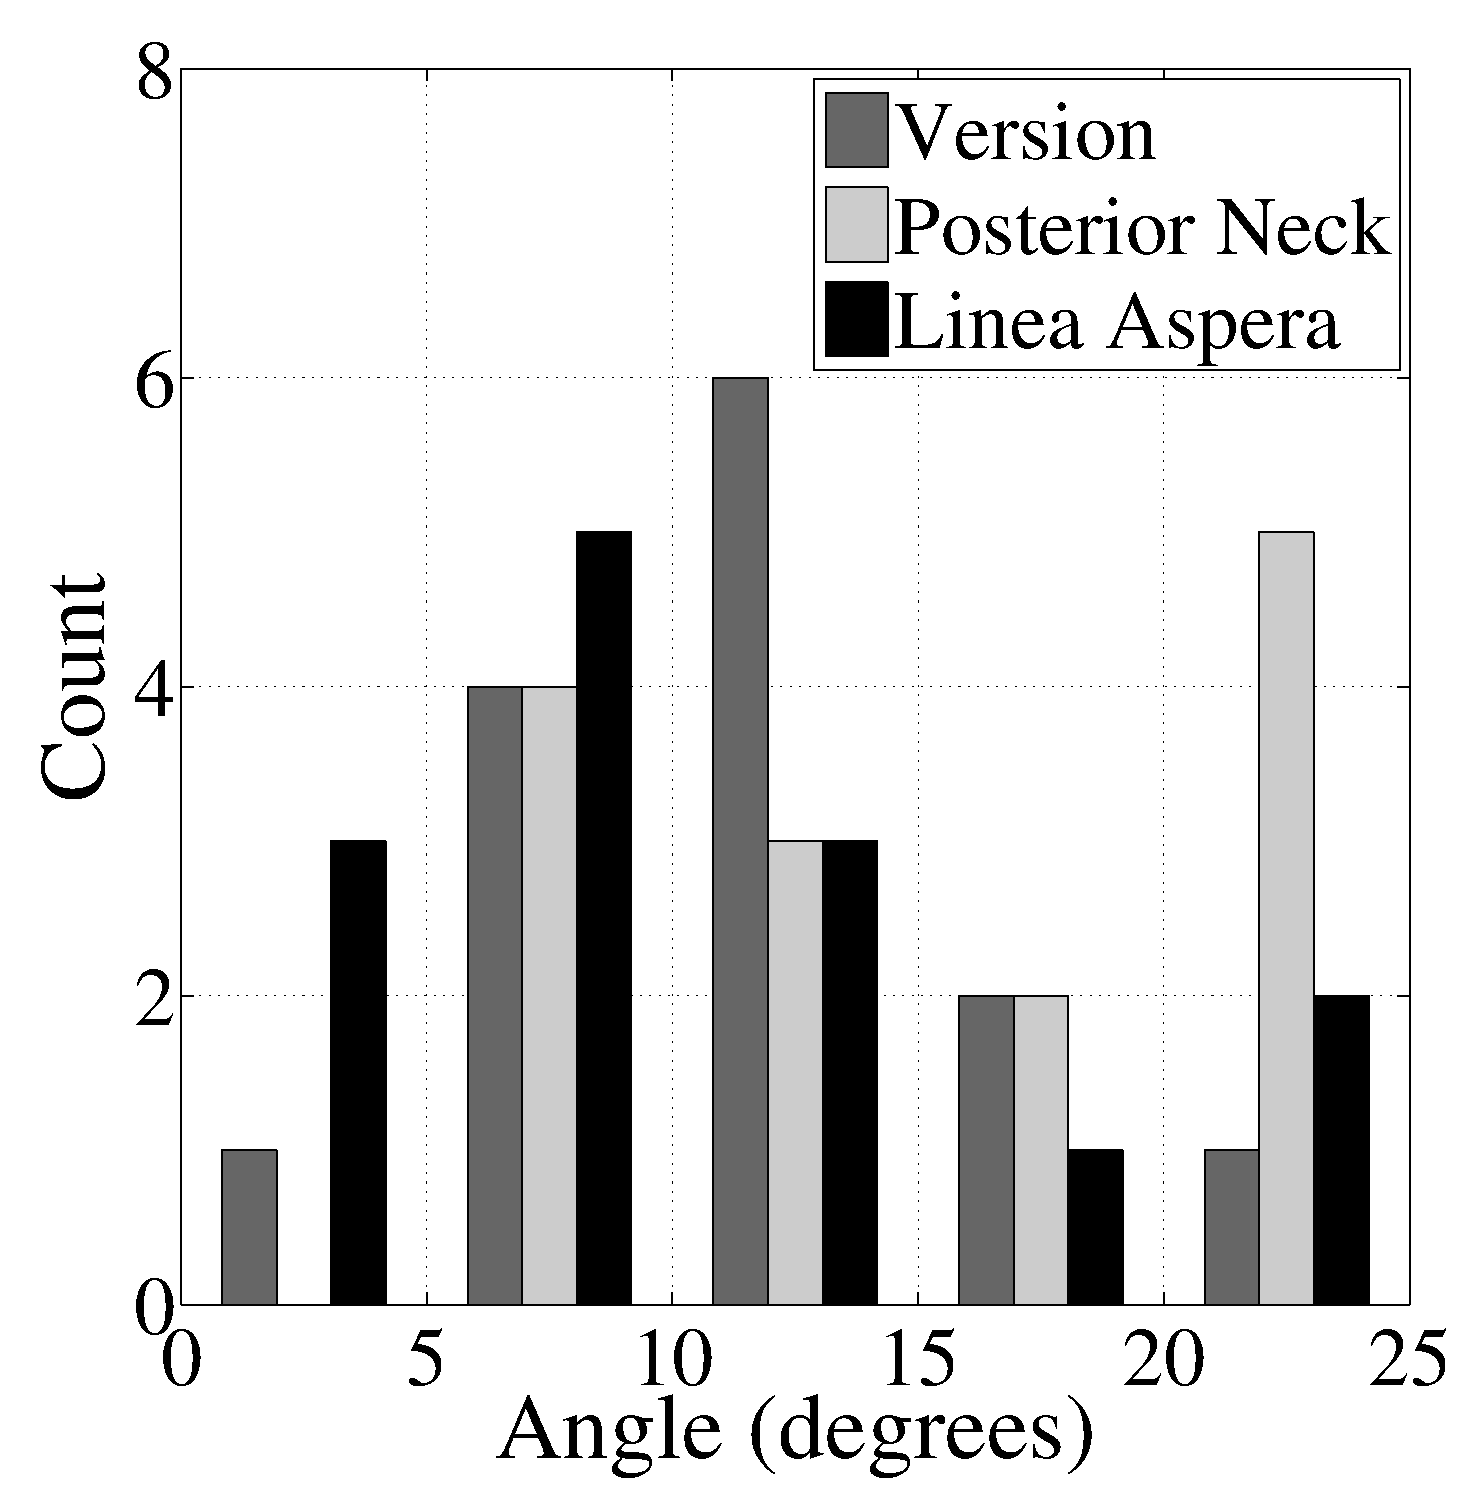
\includegraphics[width=0.7\linewidth]{./appendixVersion/figures/Distributions}
\caption[Linea aspera, version and posterior neck angle histogram]{\textbf{Distribution of version and linea aspera angles for the 14 specimens.} Graphic \copyright Seth Gilchrist, 2013.}
\label{fig:version_Distributions}
\end{figure}

\begin{figure}
\centering
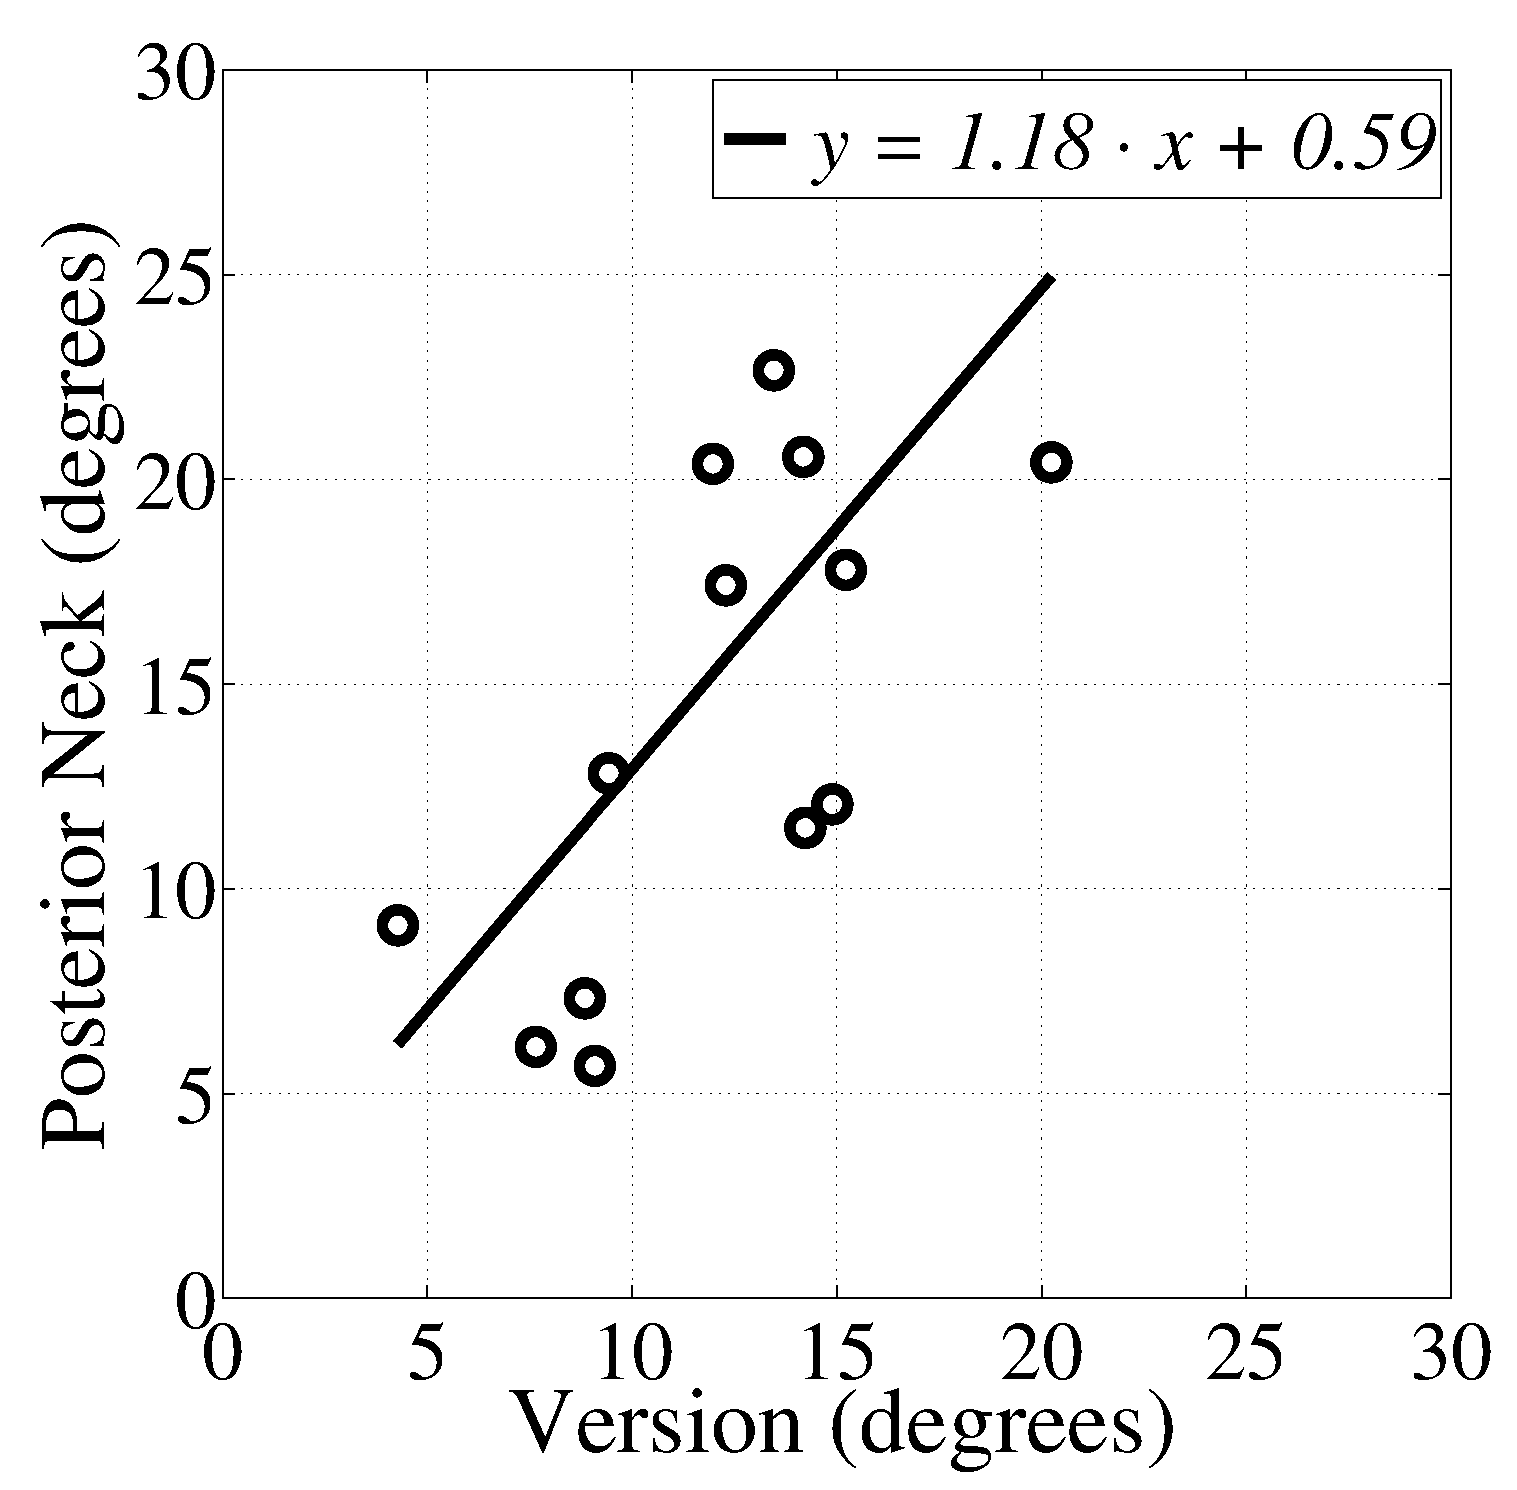
\includegraphics[width=0.7\linewidth]{./appendixVersion/figures/VersionVSPN}
\caption[Posterior neck \acs*{vs} version]{\textbf{Posterior neck angle vs.\ femoral version ($R^2 = 0.52$, $p = 0.004$).} Graphic \copyright Seth Gilchrist, 2013.}
\label{fig:version_VersionVSPN}
\end{figure}

The linea aspera angle was inversely correlated with version, meaning that as the femoral neck rotated clockwise around the shaft, the linea aspera rotated counter clockwise (Fig.~\ref{fig:version_VersionVSLA}).
This result indicates that the lateral muscles of the leg might have more impact on the location of the linea aspera than those on the medial side.
As the version increases, the shaft of the femur would tend to shift posteriorly relative to the acetabulum.
If the medial muscles drove the position, then one might expect the linea aspera to move medially, and if the lateral muscles dictate its position, one would expect it to move laterally.

\begin{figure}
\centering
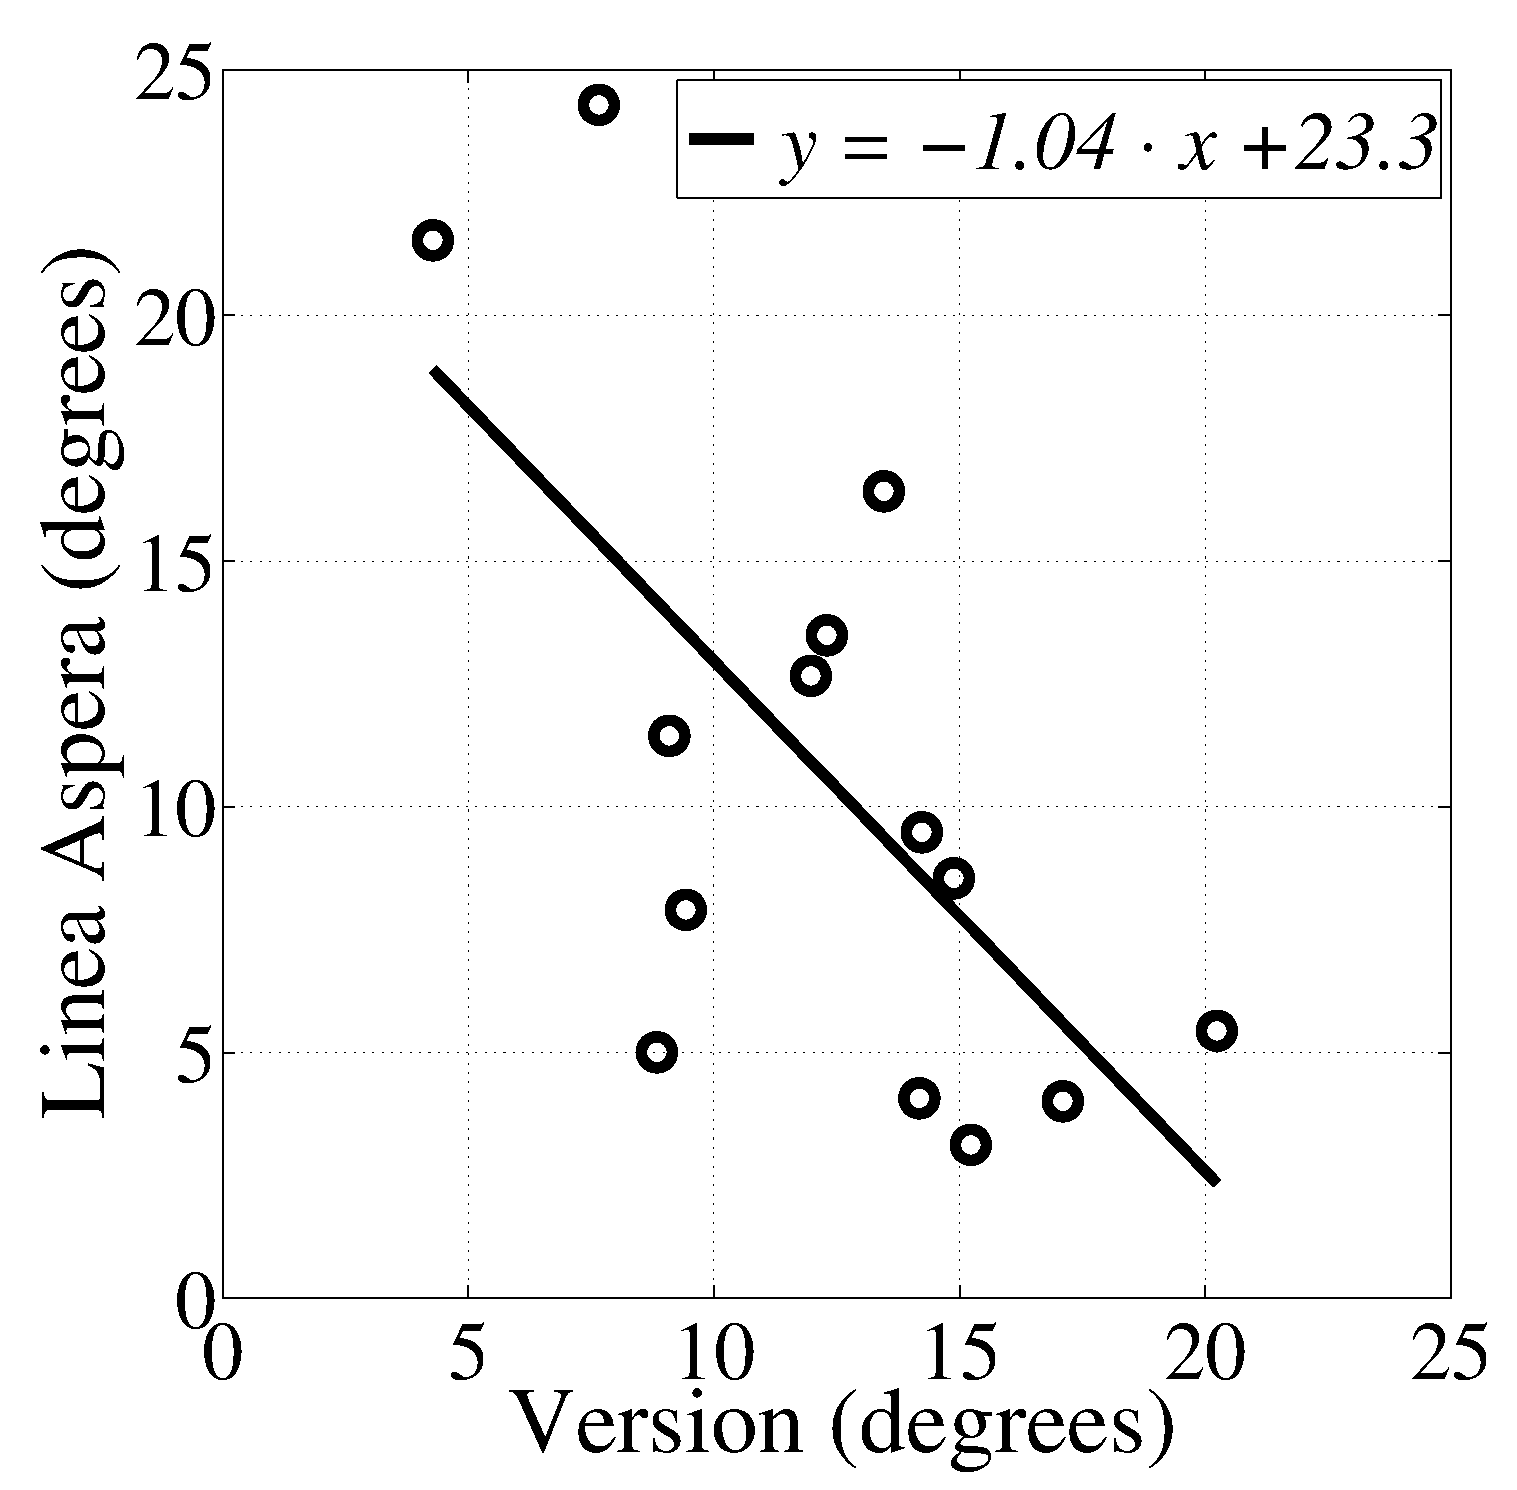
\includegraphics[width=0.7\linewidth]{./appendixVersion/figures/VersionVSLA}
\caption[Linea aspera \acs*{vs} version]{\textbf{Femoral version vs.\ linea aspera angle. ($R^2 = 0.48$, $p = 0.082$).} Graphic \copyright Seth Gilchrist, 2013.}
\label{fig:version_VersionVSLA}
\end{figure}

The separation angle between the femoral neck axis and the linea aspera increased as version increased with a slope of about 2:1 (Fig.~\ref{fig:version_VersionVSSeparation}).
This result is a mathematical consequence of the angle between the two being inversely related (Equation~\ref{equ:version_relation}).
Additionally, because the conversion from linea aspera to separation angle has a higher slope, this compresses the data in the \textit{x}-direction, which has the effect of increasing the correlation coefficient.

\begin{eqnarray}
 \ac{ala}  &=& -1.04 \cdot \ac{av} +23.3 \nonumber \\
 \ac{asep} &=& \ac{av}+90-\ac{ala} \nonumber\\
 \Rightarrow \ac{ala} &=& \ac{av}+90-\ac{asep} \nonumber \\
 \therefore \ac{av}+90-\ac{asep} &=&  -1.04 \cdot \ac{av}+23.3 \nonumber\\
 \ac{asep} &=& 2.04 \cdot \ac{av} +66.7 \label{equ:version_relation}
\end{eqnarray}

\begin{figure}
\centering
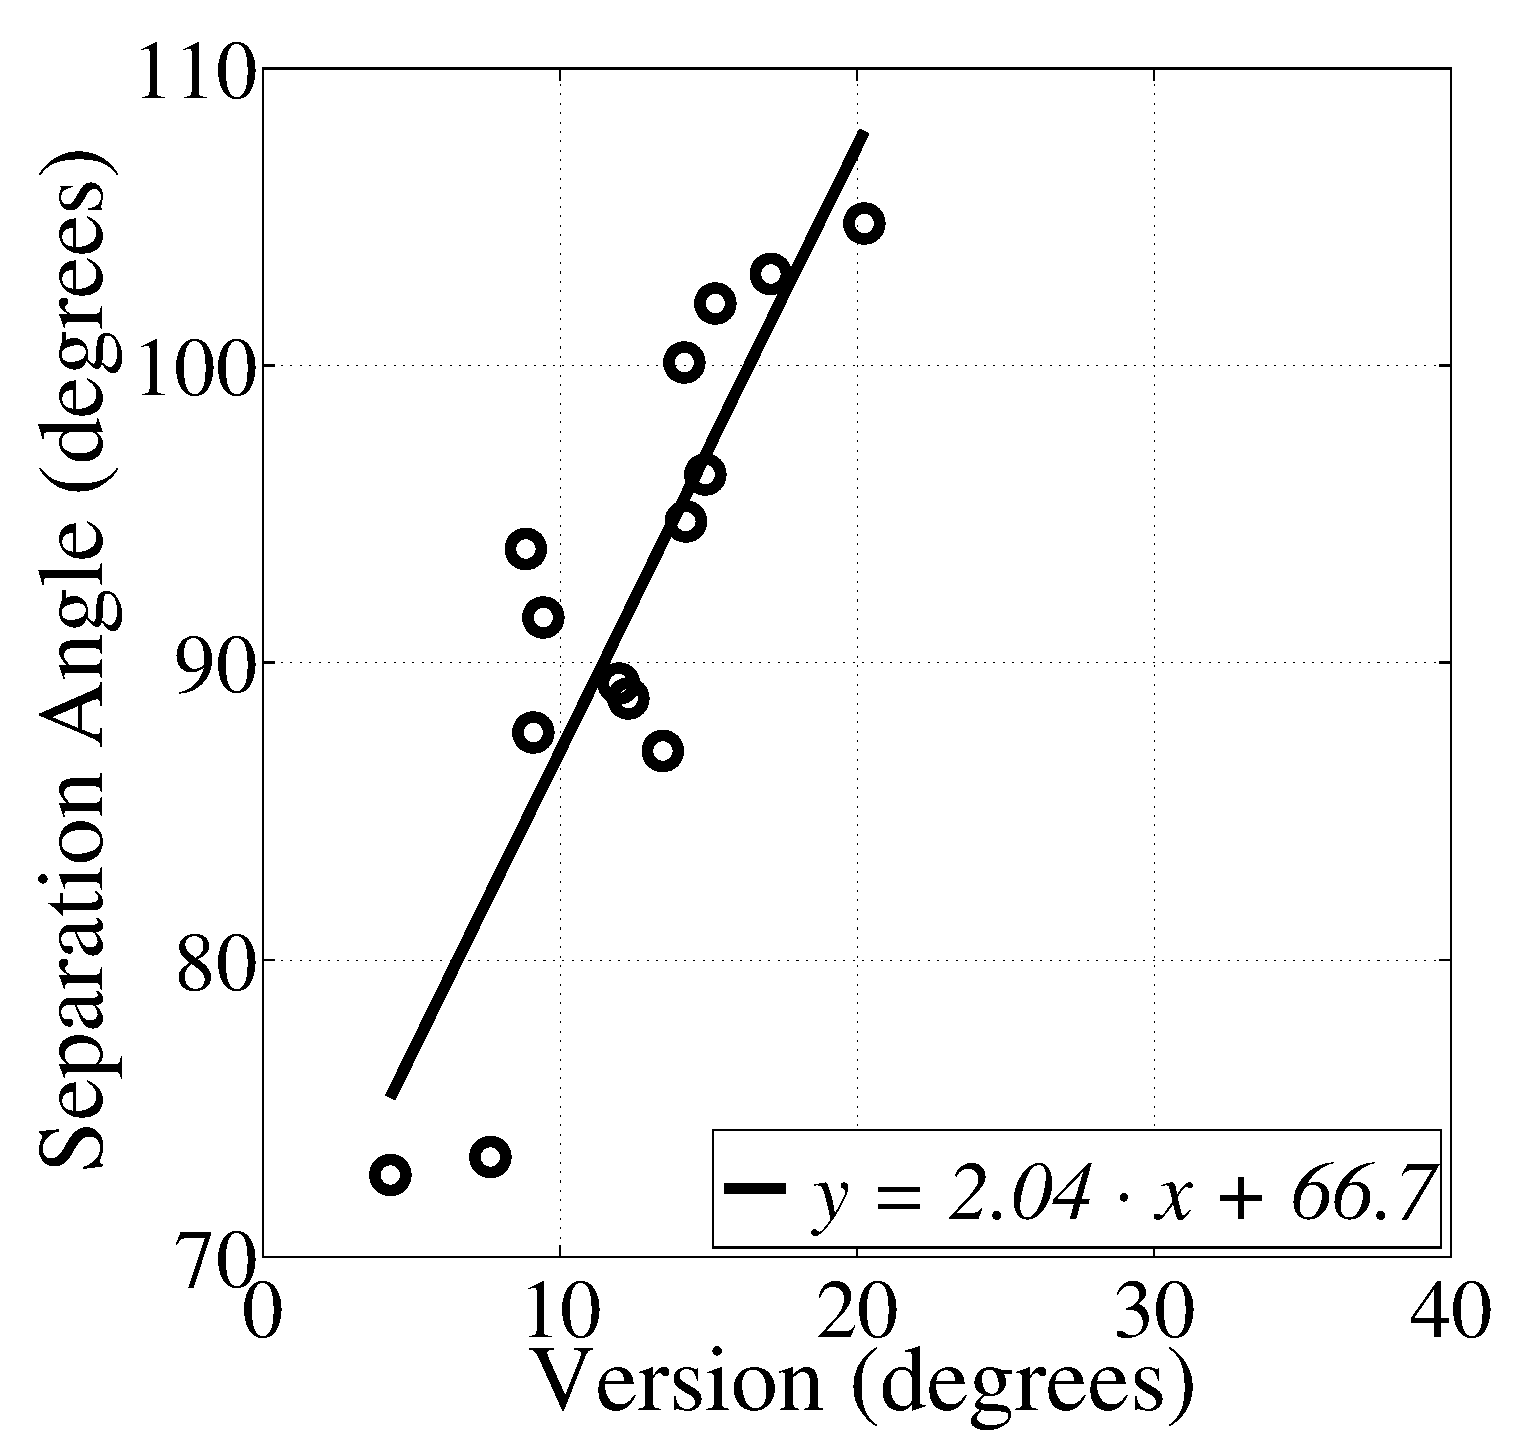
\includegraphics[width=0.7\linewidth]{./appendixVersion/figures/VersionVSSeparation}
\caption[Separation angle \acs*{vs} version]{\textbf{Femoral version vs.\ separation angle ($R^2 = 0.74$, $p = 0.0025$).} Graphic \copyright Seth Gilchrist, 2013.}
\label{fig:version_VersionVSSeparation}
\end{figure}

\section{Discussion}
\label{sec:version_discussion}
This research sought to find a relationship between the linea aspera angle and the femoral version angle.
Because the two are inversely related, the separation angle changes a version changes.
These results lead us to reject the null hypothesis and conclude that the version angle can be determined based on the separation angle, allowing researchers to determine a likely value of femoral version by measuring the angle separating the 50\% shaft linea aspera and the femoral neck.

Version values measured in our specimen group compare well with the previously published literature.
The exact origins of our specimens are unknown due to the University of British Columbia Anatomy department not collecting donor data when the specimens were originally obtained (1950's), but it was reported to the authors that they are believed to be from a South Asian population.
\citet{jain_anteversion_2003} measured version angles in 300 South Asian femora and found an average of 8.1$^\circ$ $\pm$ 6.6$^\circ$ (range = -17.2$^\circ$ to 36.7$^\circ$) using the Kingsley-Olmsted method.
\citet{khang_study_2003} measured version angles of 200 Korean femora and found an average angle of 17.9$^\circ$ $\pm$ 10.7$^\circ$ using CT scan data.
Our average version value lies between and within one standard deviation of these studies.

The correlation coefficient of 0.48 does not signify a relationship strong enough to determine one angle based on the value of the other, however, it does allow for stratification of specimens based on normal or extreme version angles.
Combining our relationship with the larger bone database analysed by \citet{jain_anteversion_2003}, if the separation angle is between 70$^\circ$ and 97$^\circ$ a specimen of South Asian origins can be considered to have a normal version, specimens with separation angles outside of these bounds should be considered to have possible extreme version angles.
During mechanical testing of femurs, this approach would allow those specimens thought to have abnormal anatomical characteristics to be identified during analysis.

The use of proximal landmarks to determine femoral version is not limited to mechanical testing of femurs.
One could consider using this reference clinically where version needs to be determined in the absence of usual proximal and distal landmarks.
This kind of situation could arise in extreme trauma where the proximal or distal ends of both femurs have been damaged and preoperative measurement of contralateral femoral version is not possible.
Additionally, in cases of metastatic cancer that require resection of the entire proximal femur, it me be possible to align the femoral arthroplasty component based on the more proximal linea aspera.

While the work provides an insight into the potential to determine femoral version using the linea aspera, there are a few limitations which must be considered before application.
First is the limited sample size, with only 14 specimens this study lacks the statistical power needed to provide a robust method for use outside of the research arena.
Additionally, the limited knowledge of the specimen population casts doubt on the applicability of these data to a wider population.
However, the consistency of the relationship in this study indicates that it is worth further investigation.
A final limitation was that the digital method of version measurement was not compared directly to a photographic method, like that used by \citet{toogood_proximal_2009} and \citet{kingsley_study_1948}.
That said, the method used in this research was modelled directly off the Kingsley-Olmsted method and is functionally the same, representing only a minor modification.

This paper provides data allowing hip fracture researchers to determine if a specimen has a potentially extreme femoral version.
This is important because it may change the orientation of the neck to the loading vector during a fall, and may also influence bone remodelling due to different lines of action of forces in hips with extreme version angles.
While the authors would not currently recommend altering the orientation used in proximal femur testing, stratification of data based on normal and extreme version could help to identify if the dearth of knowledge of specimen version is limiting our ability to determine what makes a specific femur susceptible to low trauma fracture.


\section{Acknowledgements}
\label{sec:version_acknowledge}
We thank the Centre for Hip Health and Mobility for use of their equipment, specifically the Konica-Minolta Vivid i9 scanner and the University of British Columbia for access to their historical bone collection.
